%%%%%%%%%%%%%%%%%%%%%%%%%%%%%%%%%%%%%%%%%%%%%%%%%%%%%
\section{Comparison with 27 TeV HE-HLC}
\label{sec:ana27tev}
A comparison with HE-LHC scenario has been performed.
In order to achieve it all the samples have been rederived with the associated expected energy of 27 TeV and the benchmark luminositiy used is 15 $a^{-1}$ .
\newline
The analyses strategies are the same, only the thresholds have been updated for the 27 TeV conditions. Here is the detail of the changes done :
\begin{itemize}
\item \Zpee\ or \Zpmumu : leton $p_T$ lowered from 1TeV to 0.5 TeV,
\item \Zpmumu\ f.a. and t-channel LQ : leton $p_T$ lowered from  1.2 TeV to 0.75 TeV,
\item \Zptata\ : optimal cuts changed as shown in Table~\ref{tab:leptonicresonances:selectiontautau27},
\item \rsg\ : $Jet^{trk02}(p_T^{SD Corr})$ lowered from 3 TeV to 1 TeV,
\item \Zptt\ : $Jet^{trk02}(p_T^{SD Corr})$ lowered from 3 TeV to 1 TeV,
\item \qjj\ : $Jet^{calo04}(p_T)$ lowered from 3 TeV to 1 TeV.
\end{itemize}

Table~\ref{tab:27vs100} shows the detailed results of the limit and discovery reach at $5\sigma$ for the HE-LHC 27 TeV and FCC-hh 100 TeV scenarios.
The discovery potential comparison can be found in Figure~\ref{figure:resonances27comp100:summary}.
More detailed results can be found for each 27 TeV analysis in Appendix~\ref{appendix:zpll27},~\ref{appendix:zpmumufalvano27},~\ref{appendix:zptautau27},~\ref{appendix:zptt27},~\ref{appendix:rsgww27}  and~\ref{appendix:qstarjj27}.

\begin{table}[htbp]
   \centering
\begin{tabular}{|l|l|c|r|}
  \hline
  \hline
   $\Zp$ mass [TeV] &  $\Delta \phi(\tau_1, \tau_2)$&  $\Delta R(\tau_1, \tau_2)$ & $\met$\\
  \hline
   $2$ & > 2.4 & > 2.4 and < 3.9 & > 80 GeV\\
   $4$ & > 2.4 & > 2.7 and < 4.4 & > 80 GeV\\
   $6$ & > 2.4 & > 2.9 and < 4.4 & > 80 GeV\\
   $8$ & > 2.6 & > 2.9 and < 4.6 & > 80 GeV\\
  $10$ & > 2.8 & > 2.9 and < 4.1 & > 60 GeV\\
  $12$ & > 2.8 & > 3.0 and < 3.6 & > 60 GeV\\
  $14$ & > 3.0 & > 3.0 and < 3.3 & > 60 GeV\\
  \hline
  \hline
  \end{tabular}
  \caption{List of mass dependent cuts optimised to maximise the sensitivity for the \Zptata\ search.}
  \label{tab:leptonicresonances:selectiontautau27}
\end{table}

\begin{table}[!htb]\centering
\begin{tabular}{|c|c|c|c|}
\hline
\hline
analysis   & \multicolumn{3}{c|}{HE-LHC (FCC-hh)} \\
           & Limit [TeV] & Disco [TeV]   & Disco [TeV] \\
           &             & 1 (2.5) $ab^{-1}$ & 15 (30) $ab^{-1}$ \\
\hline
\Zpee+\Zpmumu & 13 (40) & 10 (33) & 13 (43) \\
\Zptata       &  6 (14) &  3 (12) &  6 (18) \\
\Zpmumu\ f.a. &  4 (25) &  - (10) &  2 (19) \\
\Zptt         & 10 (28) &  6 (16) &  8 (23) \\
\rsg          &  8 (28) &  5 (15) &  7 (22) \\
\qjj          & 14 (43) & 10 (36) & 12 (40) \\
\hline
\hline
\end{tabular}
\caption{Limit and discovery reach at 5 $\sigma$ comparison between HE-LHC (27 TeV 15 ab-1) and FCC-hh (100 TeV 30 ab-1).}
\label{tab:27vs100}
\end{table}

\begin{figure}[!htb]
  \centering
  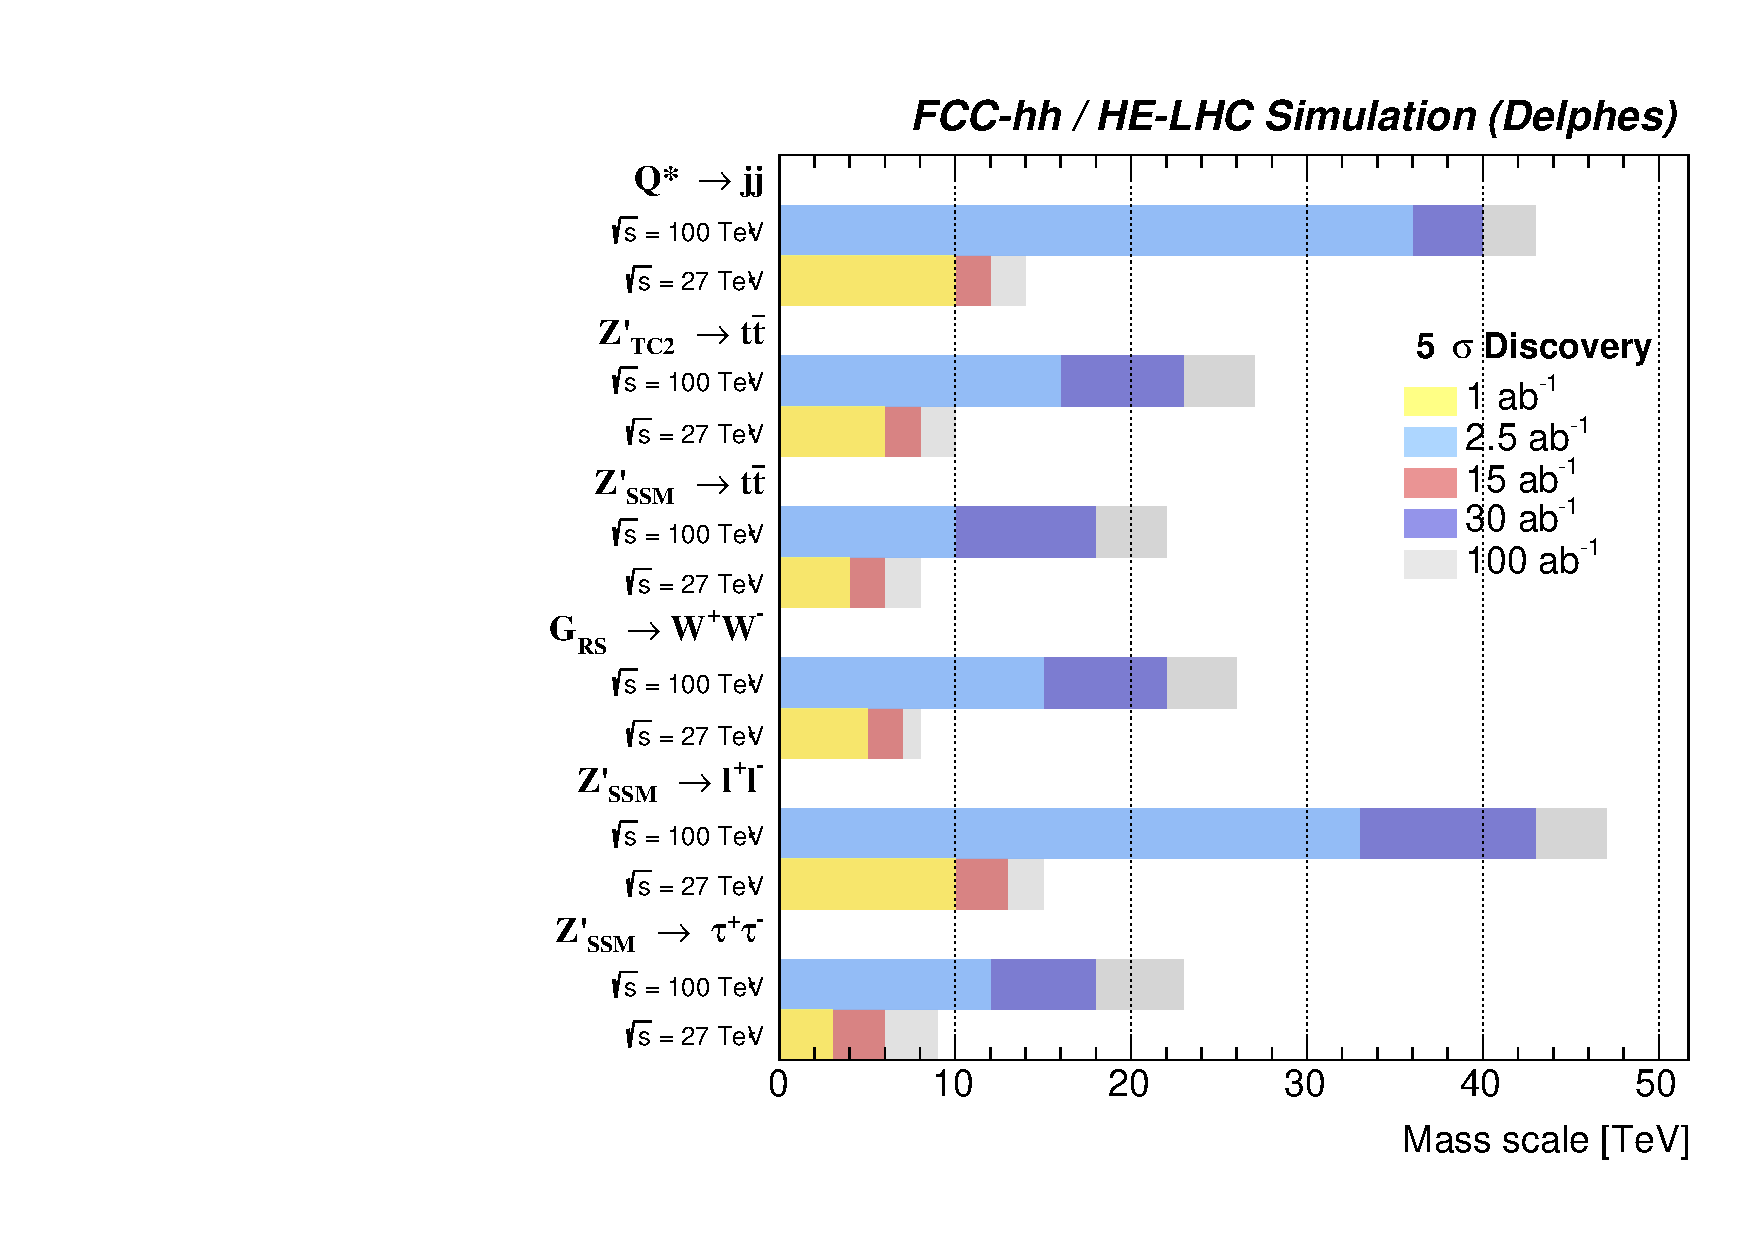
\includegraphics[width=0.90\columnwidth]{Fig/summaryDisco.pdf}
  \caption{Summary of a $5\sigma$ discovery reach as a function of the resonance mass for different luminosity scenario of FCC-hh and HE-LHC.}
  \label{figure:resonances27comp100:summary}
\end{figure}